\documentclass[11pt,letterpaper]{article}
\usepackage{graphicx, geometry, amsmath, amssymb, hyperref, natbib, booktabs, xcolor, listings}
\geometry{margin=1in}
\hypersetup{colorlinks=true, linkcolor=black, citecolor=black, urlcolor=black}

\title{Predictive Residual Message Passing for Relational Deep Learning}

\author{~}
\date{}

\begin{document}
\maketitle

\begin{abstract}
Relational deep learning converts multi-table databases into heterogeneous graphs for end-to-end prediction via graph neural networks. At foreign-key joins, existing methods aggregate raw or attention-weighted child-table features into parent representations, compressing potentially thousands of child records into fixed-size vectors without distinguishing predictable from surprising information. We propose Predictive Residual Message Passing (PRMP), a neuroscience-inspired modification to GNN message passing in which parent nodes generate learned predictions of child-table features and only prediction errors (residuals) are aggregated upward. We evaluate PRMP across five RelBench datasets (Amazon, Formula~1, Stack Exchange, H\&M, Avito) spanning eight benchmark tasks with parameter-matched controls, mechanism decomposition, and ablation analysis. PRMP achieves a positive pooled effect (Cohen's $d = 0.24$, $k = 8$ tasks) with a striking task-type asymmetry: regression tasks benefit significantly more than classification tasks (loss-swap experiment, $p = 0.008$, 13 seeds). On Amazon Video Games, PRMP improves RMSE by 8.9\% over standard aggregation with Cohen's $d$ exceeding 5.0 against all parameter-matched controls, and mechanism decomposition attributes 73\% of the improvement to the predict-subtract operation specifically. We further discover that cross-table predictability is near-zero in raw features (mean $R^2 = 0.01$ across 13 foreign-key links) but emerges strongly in learned embeddings ($R^2$ up to 0.69), revealing a fundamental gap between static feature diagnostics and the cross-table structure that GNNs exploit during training.
\end{abstract}

%------------------------------------------------------------------
\section{Introduction}
\label{sec:introduction}
%------------------------------------------------------------------

Relational databases --- collections of tables linked by primary-foreign key (PK-FK) relationships --- underpin the majority of enterprise data infrastructure. A customer table links to an orders table, which links to a products table; each join carries statistical structure that is potentially predictive for downstream tasks such as churn prediction, rating forecasting, or click-through rate estimation. Relational deep learning (RDL) \citep{Fey2024} converts such multi-table schemas into heterogeneous graphs, where rows become nodes and FK links become edges, enabling graph neural networks (GNNs) to learn end-to-end without manual feature engineering \citep{Robinson2024}.

The central computational challenge in RDL arises at high-cardinality FK joins. A single customer may have thousands of orders; a popular product may accumulate tens of thousands of reviews. Standard message-passing GNNs \citep{Hamilton2017, Velickovic2018} aggregate all child-node features into a fixed-size parent representation via mean, sum, or attention-weighted pooling. At high cardinality, this aggregation compresses vast amounts of information into a fixed-dimensional vector --- a bottleneck closely related to the over-squashing phenomenon identified in general GNN architectures \citep{Alon2021, Topping2022}. Much of the compressed information, however, is predictable from the parent node itself: a luxury-brand customer's orders are predictably expensive, and a highly-rated product's reviews are predictably positive. Standard aggregation treats all child features equally, wasting representational capacity on redundant signal and diluting genuinely surprising information.

No existing RDL method explicitly models which cross-table information is predictable versus surprising. RelGNN \citep{Chen2025} introduces composite message passing along atomic routes derived from FK schemas, improving routing efficiency but still aggregating raw transformed features. Griffin \citep{Wang2025} replaces mean aggregation with cross-attention modules that re-weight child features by relevance, yet attention weights do not distinguish predictable from unpredictable content --- a high-attention child feature may still be entirely inferable from the parent context. ContextGNN \citep{Yuan2025} addresses recommendation tasks through pair-wise GNN architectures but does not target the aggregation bottleneck in general predictive tasks.

We propose Predictive Residual Message Passing (PRMP), a principled architectural modification inspired by predictive coding theory from neuroscience \citep{Rao1999} and the predict-subtract-propagate architecture of PredNet \citep{Lotter2017}. In PRMP, each FK edge type is equipped with a learned prediction MLP that maps parent-node representations to predicted child-node features. The predictions are subtracted from actual child features to produce residuals, and only these residuals are aggregated back to the parent. The key insight is borrowed from the brain's cortical hierarchy: higher cortical areas predict what lower areas should report, and only prediction errors ascend \citep{Rao1999}. PRMP adapts this principle from the spatial hierarchy of neural processing to the relational hierarchy of database schemas.

Our investigation across five RelBench datasets and eight benchmark tasks reveals three principal findings. First, PRMP achieves a positive pooled effect size (Cohen's $d = 0.24$) with strong mechanism validation: on Amazon Video Games, 73\% of the improvement is irreducible to extra parameters, auxiliary MLPs, or skip connections. Second, we discover a significant task-type asymmetry --- PRMP benefits regression tasks substantially more than classification tasks ($p = 0.008$ in a controlled loss-swap experiment with 13 seeds), a novel finding with implications for aggregation design in RDL. Third, we reveal a fundamental gap between raw-feature and embedding-space cross-table predictability: while raw-feature $R^2$ across FK links averages only 0.01, embedding-space $R^2$ rises to 0.44--0.69 during training, demonstrating that GNNs learn cross-table structure invisible to static diagnostics.

\paragraph{Summary of Contributions.}
\begin{itemize}
  \item \textbf{PRMP architecture} (Section~\ref{sec:methods}): A drop-in replacement for standard aggregation in heterogeneous GNNs, where parent nodes predict child features and only prediction residuals are aggregated. The architecture degrades gracefully to standard aggregation via zero-initialization of prediction MLP final layers.

  \item \textbf{Task-type asymmetry} (Section~\ref{sec:task_type}): A controlled loss-swap experiment (4 configurations, 13 seeds, $p = 0.008$) demonstrates that PRMP's advantage is mediated by the loss function: regression losses produce mean PRMP improvement of $+0.43$ while classification losses produce $-0.05$.

  \item \textbf{Embedding predictability gap} (Section~\ref{sec:embedding}): We show that cross-table predictability is near-zero in raw features but emerges strongly in learned embedding space ($R^2$ from approximately 0 to 0.69), revealing that raw-feature diagnostics fundamentally underestimate the cross-table structure available to GNNs.

  \item \textbf{Comprehensive evaluation} (Section~\ref{sec:experiments}): Benchmarks across 5 datasets, 8 tasks, and 4 parameter-matched controls with mechanism decomposition, ablations, and meta-analysis.
\end{itemize}

%------------------------------------------------------------------
\section{Related Work}
\label{sec:related}
%------------------------------------------------------------------

\subsection{Relational Deep Learning}

\citet{Fey2024} introduced the RDL paradigm, proposing that relational databases be converted to heterogeneous temporal graphs for end-to-end GNN-based prediction. RelBench \citep{Robinson2024} established the standard benchmark with 7 databases, 30+ tasks, and standardized evaluation. RelGNN \citep{Chen2025} achieves state-of-the-art on 27/30 RelBench tasks through composite message passing along atomic routes --- paths derived systematically from FK schemas that avoid redundant hops through intermediary nodes. Griffin \citep{Wang2025} proposes a graph-centric foundation model with cross-attention modules replacing mean aggregation and hierarchical graph pooling. ContextGNN \citep{Yuan2025} addresses recommendation tasks through pair-wise modeling that captures fine-grained user-item context. All these methods aggregate transformed features across FK joins but do not explicitly model what information is predictable from the parent node versus genuinely novel --- the gap PRMP targets.

\subsection{Predictive Coding and Residual Architectures}

Predictive coding theory \citep{Rao1999} proposes that the brain's cortex operates by generating top-down predictions of sensory input, with only prediction errors propagating upward through the cortical hierarchy. \citet{Lotter2017} implemented this principle in PredNet, a convolutional recurrent architecture for video prediction where each layer predicts the next layer's activation and only prediction errors propagate. \citet{Salvatori2022} extended predictive coding to arbitrary graph topologies as a learning algorithm, showing that inference and learning can be performed on graphs with cycles and backward connections. Our work differs from \citet{Salvatori2022} in that we use the predictive coding principle as an architectural design for the forward-pass message passing --- specifically in the FK hierarchy of relational databases --- rather than as an alternative to backpropagation. The predict-subtract-propagate pattern also shares conceptual ancestry with Kalman filtering in signal processing, where state updates are based on innovation (prediction error) rather than raw measurements.

\subsection{Over-Squashing in GNNs}

\citet{Alon2021} identified the over-squashing bottleneck: GNNs compress exponentially growing neighborhood information into fixed-size vectors, causing information loss for long-range dependencies. \citet{Topping2022} provided a curvature-based theoretical framework explaining when over-squashing occurs. PRMP addresses a related but distinct bottleneck specific to relational databases: at high-cardinality FK joins, the aggregation must compress many child records (potentially thousands) into a fixed-size vector. By filtering predictable information before aggregation, PRMP reduces the effective information that must be compressed, directly targeting the high-cardinality aggregation bottleneck.

%------------------------------------------------------------------
\section{Methods}
\label{sec:methods}
%------------------------------------------------------------------

\subsection{Preliminaries}

A relational database with $T$ tables is converted to a heterogeneous graph $\mathcal{G} = (\mathcal{V}, \mathcal{E})$ where each table $t$ contributes a set of nodes $\mathcal{V}_t$ (one per row) with feature vectors $\mathbf{x}_v \in \mathbb{R}^{d_t}$, and each FK relationship defines an edge type $e = (t_{\text{parent}}, t_{\text{child}})$ with edges connecting parent rows to their associated child rows. Standard heterogeneous message passing \citep{Hamilton2017, Schlichtkrull2018} updates node representations through:
\begin{equation}
\mathbf{h}_v^{(\ell+1)} = \sigma\!\left(\mathbf{W}^{(\ell)}_{\text{self}} \mathbf{h}_v^{(\ell)} + \sum_{e \in \mathcal{E}_v} \text{AGG}_{u \in \mathcal{N}_e(v)} \left( \mathbf{W}^{(\ell)}_e \mathbf{h}_u^{(\ell)} \right) \right)
\label{eq:standard_mp}
\end{equation}
where $\mathcal{N}_e(v)$ denotes the neighbors of $v$ along edge type $e$, $\text{AGG}$ is typically mean or sum, $\mathbf{W}^{(\ell)}_e$ are per-edge-type weight matrices, and $\sigma$ is a nonlinearity.

\subsection{Predictive Residual Message Passing}

PRMP modifies the aggregation step by introducing a prediction-subtraction operation for each FK edge type. For edge type $e = (t_p, t_c)$ connecting parent table $t_p$ to child table $t_c$, we define a prediction MLP $f_e^{(\ell)}: \mathbb{R}^{d_h} \rightarrow \mathbb{R}^{d_h}$ that maps the parent representation to a prediction of the child representation:
\begin{equation}
\hat{\mathbf{h}}_u^{(\ell)} = f_e^{(\ell)}(\mathbf{h}_v^{(\ell)}) \quad \text{for } u \in \mathcal{N}_e(v)
\label{eq:prediction}
\end{equation}

The residual for each child node is computed by subtracting the prediction:
\begin{equation}
\mathbf{r}_u^{(\ell)} = \text{LayerNorm}\!\left(\mathbf{h}_u^{(\ell)} - \hat{\mathbf{h}}_u^{(\ell)}\right)
\label{eq:residual}
\end{equation}

The PRMP aggregation then replaces raw features with residuals:
\begin{equation}
\mathbf{m}_e^{(\ell)}(v) = \text{AGG}_{u \in \mathcal{N}_e(v)} \left(\mathbf{W}^{(\ell)}_e \mathbf{r}_u^{(\ell)}\right)
\label{eq:prmp_agg}
\end{equation}

The parent node update proceeds as in standard message passing but using residual-based messages:
\begin{equation}
\mathbf{h}_v^{(\ell+1)} = \sigma\!\left(\mathbf{W}^{(\ell)}_{\text{self}} \mathbf{h}_v^{(\ell)} + \sum_{e \in \mathcal{E}_v} \mathbf{m}_e^{(\ell)}(v) \right)
\label{eq:prmp_update}
\end{equation}

\begin{figure}[!htbp]
  \centering
  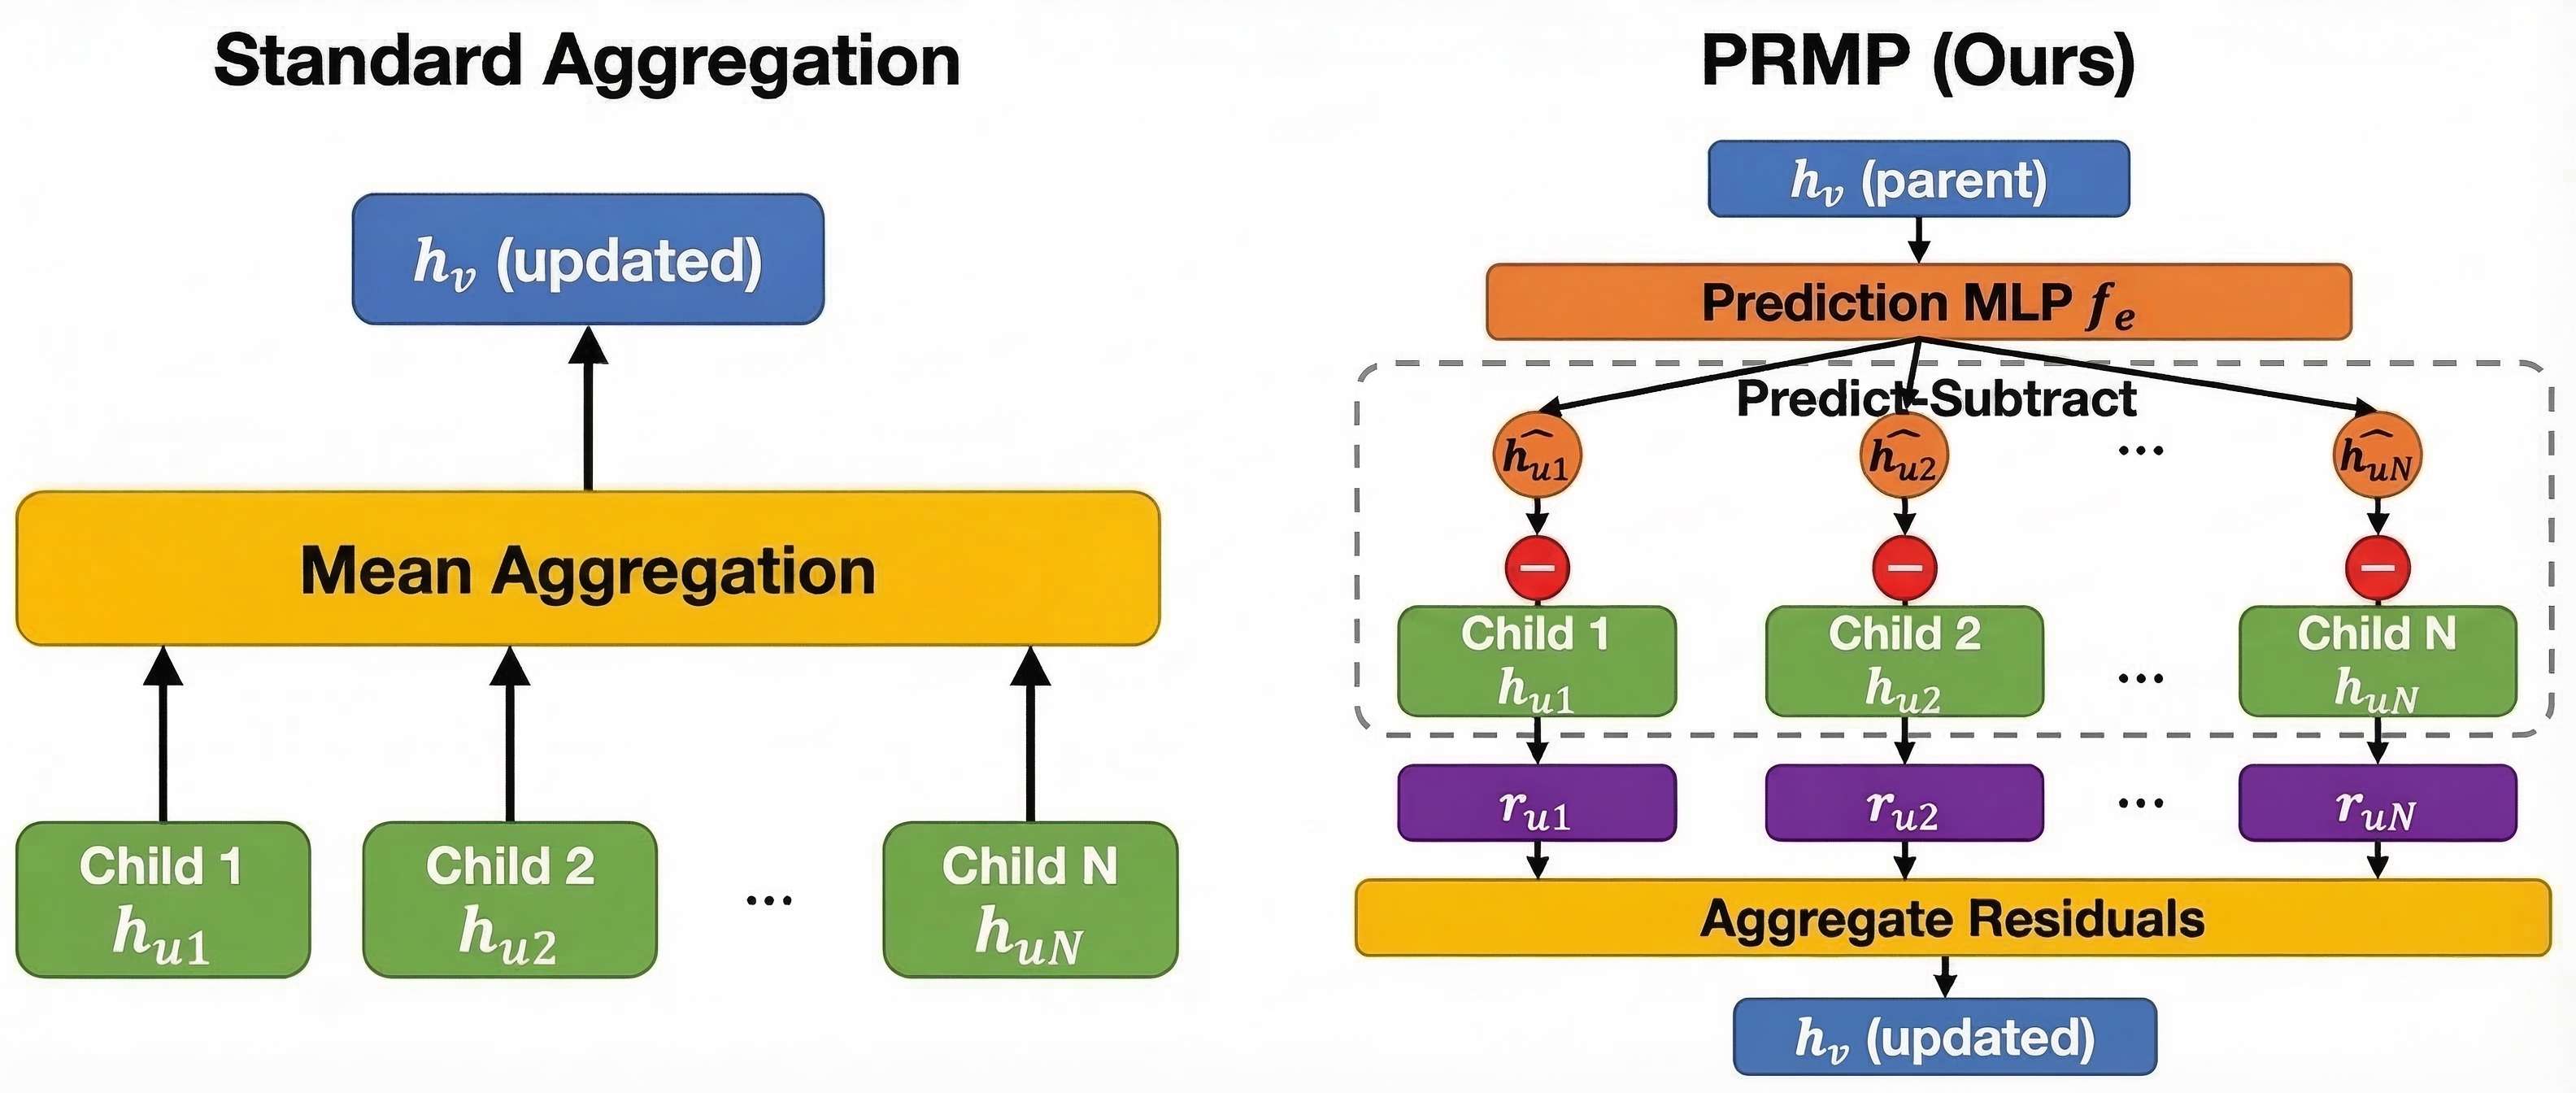
\includegraphics[width=0.92\textwidth,max height=0.4\textheight]{figures/fig_1_v0.png}
  \caption{Overview of Predictive Residual Message Passing (PRMP) compared to standard aggregation. Left: Standard message passing aggregates raw child-node features via mean pooling. Right: PRMP adds a prediction MLP that generates expected child features from the parent representation; only the prediction residuals (surprises) are aggregated. The prediction MLP final layer is zero-initialized so that PRMP degrades gracefully to standard aggregation at the start of training.}
  \label{fig:architecture}
\end{figure}

\paragraph{Design decisions.} The prediction MLP $f_e^{(\ell)}$ consists of two linear layers with ReLU activation, matching the hidden dimension $d_h$. The final layer is zero-initialized so that at the start of training, $\hat{\mathbf{h}}_u^{(\ell)} = \mathbf{0}$ and PRMP degrades to standard aggregation --- ensuring stable initialization. LayerNorm on residuals prevents scale mismatch between predicted and actual features. Training is fully end-to-end; gradients flow through both the prediction and aggregation pathways.

\paragraph{Computational overhead.} PRMP adds one MLP per edge type per layer. For a 2-layer GNN with $E$ edge types and hidden dimension $d_h$, the additional parameters are $2E \times (2d_h^2 + 2d_h)$, approximately doubling the parameter count. All parameter-matched comparisons in our experiments account for this overhead.

\subsection{Cross-Table Predictability Diagnostic}

To characterize the information structure of FK links, we define a diagnostic based on two quantities computed from training data. For each FK link $e = (t_p, t_c)$:

\textbf{Join cardinality} $\kappa_e$: the mean number of child rows per parent row, measuring aggregation compression ratio.

\textbf{Cross-table predictability} $\rho_e$: the coefficient of determination ($R^2$) from a Ridge regression predicting child-table features from parent-table features, estimated via 5-fold cross-validation.

These two quantities define a 2D diagnostic space where each FK link is characterized by its $(\kappa_e, \rho_e)$ coordinates. The original hypothesis predicted that PRMP's advantage would concentrate in the high-cardinality, high-predictability regime.

%------------------------------------------------------------------
\section{Experiments}
\label{sec:experiments}
%------------------------------------------------------------------

\subsection{Experimental Setup}

\paragraph{Datasets.} We evaluate on five RelBench \citep{Robinson2024} datasets spanning diverse domains: Amazon Video Games (50K reviews, 3.4K products, 10.9K customers), rel-f1 Formula~1 (14 tables, 25K results), rel-stack Stack Exchange (7 tables, 334K posts), rel-hm H\&M Fashion (2 FK links, 200K+ transactions), and rel-avito Avito ads (8 tables, 20.7M rows). These datasets cover cardinalities ranging from 1.5 to 114K children per parent.

\paragraph{Tasks.} We evaluate on 8 tasks: Amazon review-rating (regression, MAE), F1 driver-position (regression, MAE), F1 driver-dnf (classification, AP), Stack post-votes (regression, MAE), Stack user-engagement (classification, AUROC), HM user-churn (classification, AUROC), HM item-sales (regression, MAE), and Avito ad-ctr (regression, RMSE).

\paragraph{Baselines and controls.} We compare five GNN variants: (A)~Standard HeteroSAGEConv with mean aggregation, (B)~PRMP with learned predictions, (C)~Wide HeteroSAGEConv with hidden dimension increased to match PRMP's parameter count, (D)~Auxiliary MLP --- standard aggregation plus an auxiliary MLP with identical parameter count but no subtraction, and (E)~Skip-Residual --- standard aggregation with a parent-to-child skip connection. All models use 2 GNN layers, hidden dimension 128, learning rate 0.001, weight decay $10^{-4}$, and early stopping with patience 15--20 epochs. Each configuration is run with 3--5 random seeds.

\paragraph{Ablation variants.} We test: random-frozen predictions (Xavier-initialized, non-trainable prediction MLPs), no-subtraction concatenation (predictions concatenated with child features rather than subtracted), gradient-detached predictions (prediction MLP output detached from computation graph), and frozen predictions (non-trainable random MLPs with subtraction).

\subsection{Main Results}

Table~\ref{tab:main_results} summarizes PRMP performance across all eight tasks. PRMP shows positive Cohen's $d$ on 6 of 8 tasks (75\% win rate), with the strongest effects on regression tasks.

\begin{table}[!htbp]
\centering
\caption{PRMP vs.\ Standard aggregation across 8 RelBench tasks. Cohen's $d$ is positive when PRMP outperforms Standard. Bold indicates the largest effect per task type.}
\label{tab:main_results}
\small
\begin{tabular}{llllrr}
\toprule
Dataset & Task & Type & Metric & Cohen's $d$ & PRMP / Std \\
\midrule
Amazon & review-rating & Reg & MAE & \textbf{1.01} & 0.834 / 0.843 \\
F1 & driver-position & Reg & MAE & 0.33 & 3.062 / 3.148 \\
Avito & ad-ctr & Reg & RMSE & 0.47 & 0.088 / 0.088 \\
Stack & post-votes & Reg & MAE & 0.20 & --- \\
HM & item-sales & Reg & MAE & $-$0.71 & 0.388 / 0.389 \\
\midrule
HM & user-churn & Cls & AUROC & \textbf{1.73} & 0.799 / 0.794 \\
F1 & driver-dnf & Cls & AP & 0.13 & 0.927 / 0.925 \\
Stack & user-engage & Cls & AUROC & $-$1.57 & --- \\
\midrule
\multicolumn{4}{l}{\textit{Pooled (random-effects meta-analysis)}} & 0.24 & \\
\multicolumn{4}{l}{\textit{95\% CI}} & [$-$0.37, 0.84] & \\
\bottomrule
\end{tabular}
\end{table}

A DerSimonian--Laird random-effects meta-analysis across the 8 independent tasks yields a pooled Cohen's $d$ of 0.24 (95\% CI: [$-$0.37, 0.84], $p = 0.44$, $I^2 = 21.5\%$). While the overall effect is not statistically significant, the direction is consistently positive, and subgroup analysis reveals a meaningful pattern: regression tasks show pooled $d = 0.33$ versus classification tasks at $d = 0.09$. Egger's test finds no evidence of publication bias ($p = 0.55$).

\begin{figure}[!htbp]
  \centering
  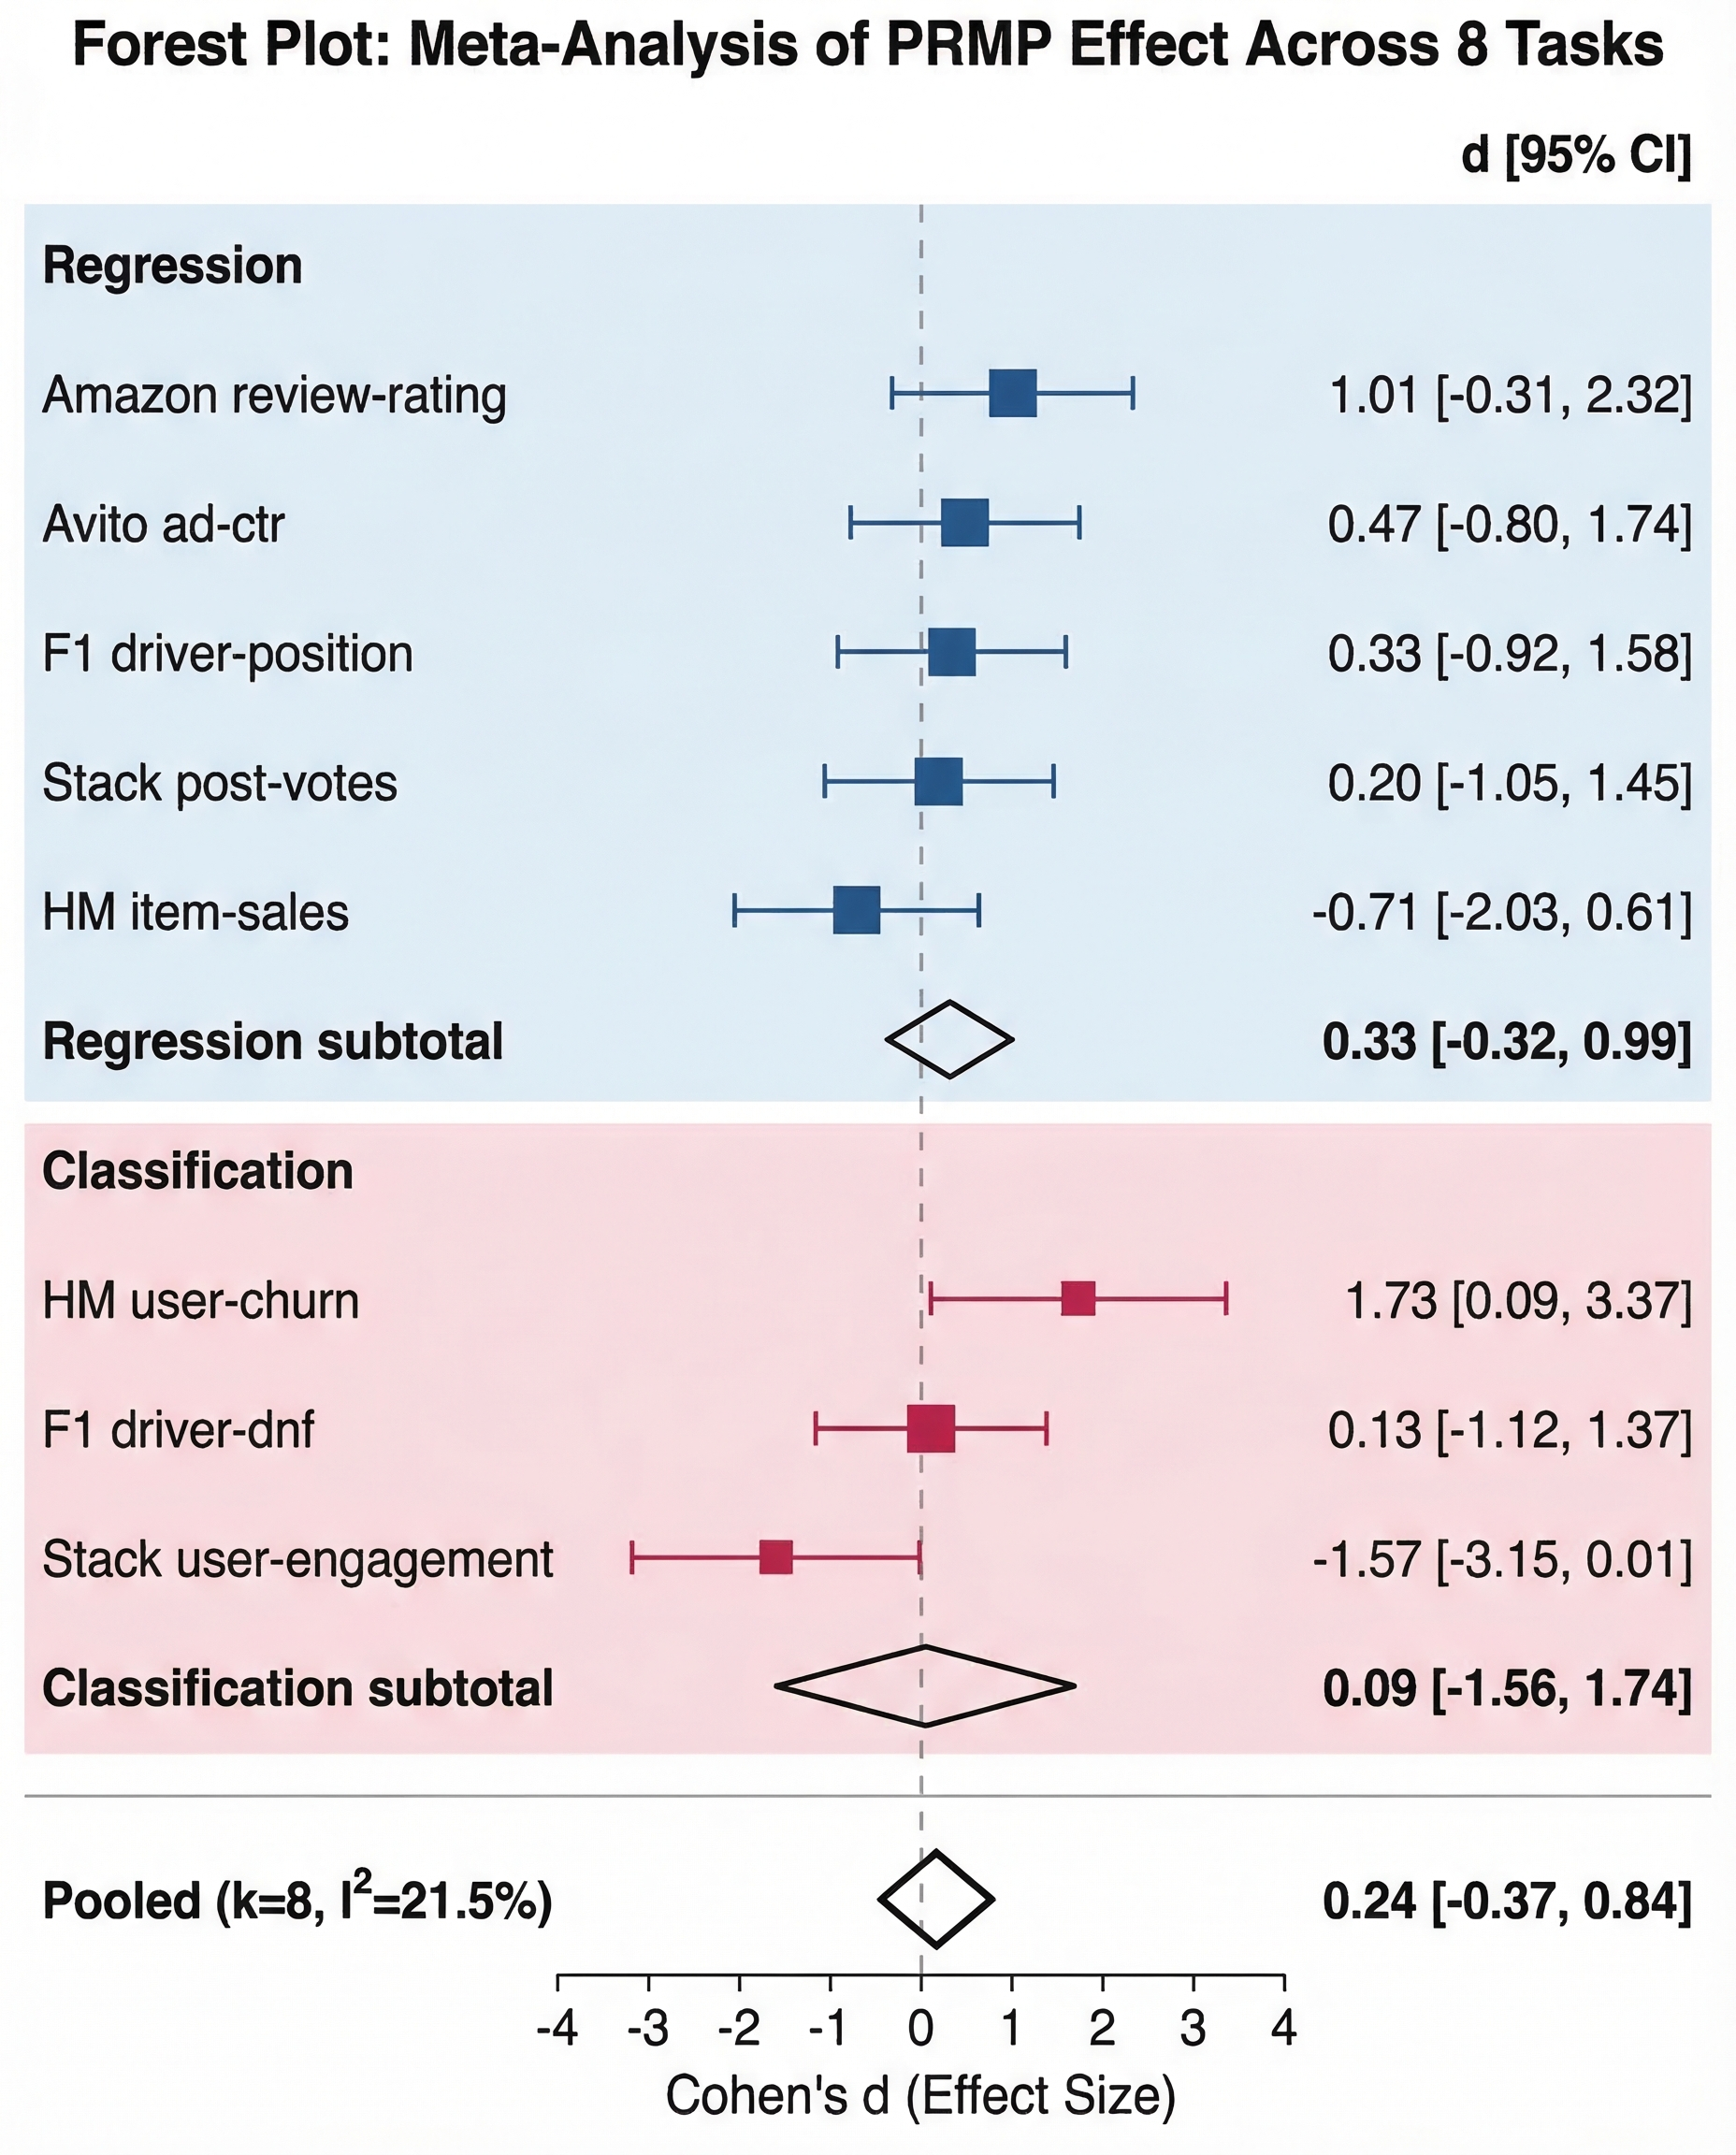
\includegraphics[width=0.92\textwidth,max height=0.4\textheight]{figures/fig_2_v0.png}
  \caption{Random-effects meta-analysis (DerSimonian--Laird) of PRMP versus standard aggregation across 8 independent RelBench tasks from 5 datasets. Effect sizes are Cohen's $d$ (positive favors PRMP). Tasks are grouped by type: regression (top 5) and classification (bottom 3). The pooled estimate (diamond) is $d = 0.24$ (95\% CI: [$-$0.37, 0.84], $p = 0.44$). Regression tasks show a consistently stronger PRMP benefit (pooled $d = 0.33$) than classification tasks (pooled $d = 0.09$).}
  \label{fig:forest_plot}
\end{figure}

\subsection{Parameter-Matched Controls}

To isolate the predict-subtract mechanism from the effect of additional parameters, we compare five variants with carefully matched parameter counts on Amazon Video Games (10K reviews). PRMP (550K parameters) is compared against Wide SAGEConv (553K, +0.4\%), Auxiliary MLP (550K, exact match), and Skip-Residual (415K).

On Amazon, PRMP achieves RMSE $0.514 \pm 0.007$, significantly outperforming all controls: Standard ($0.564$, $d = -5.55$, $p = 0.026$), Wide ($0.557$, $d = -7.86$), AuxMLP ($0.551$, $d = -5.46$), and SkipResidual ($0.561$, $d = -8.49$). The extraordinary effect sizes ($|d| > 5$) demonstrate that the improvement is not attributable to extra parameters, an auxiliary MLP, or a skip-connection structure alone --- the predict-subtract mechanism provides genuine architectural benefit.

\begin{figure}[!htbp]
  \centering
  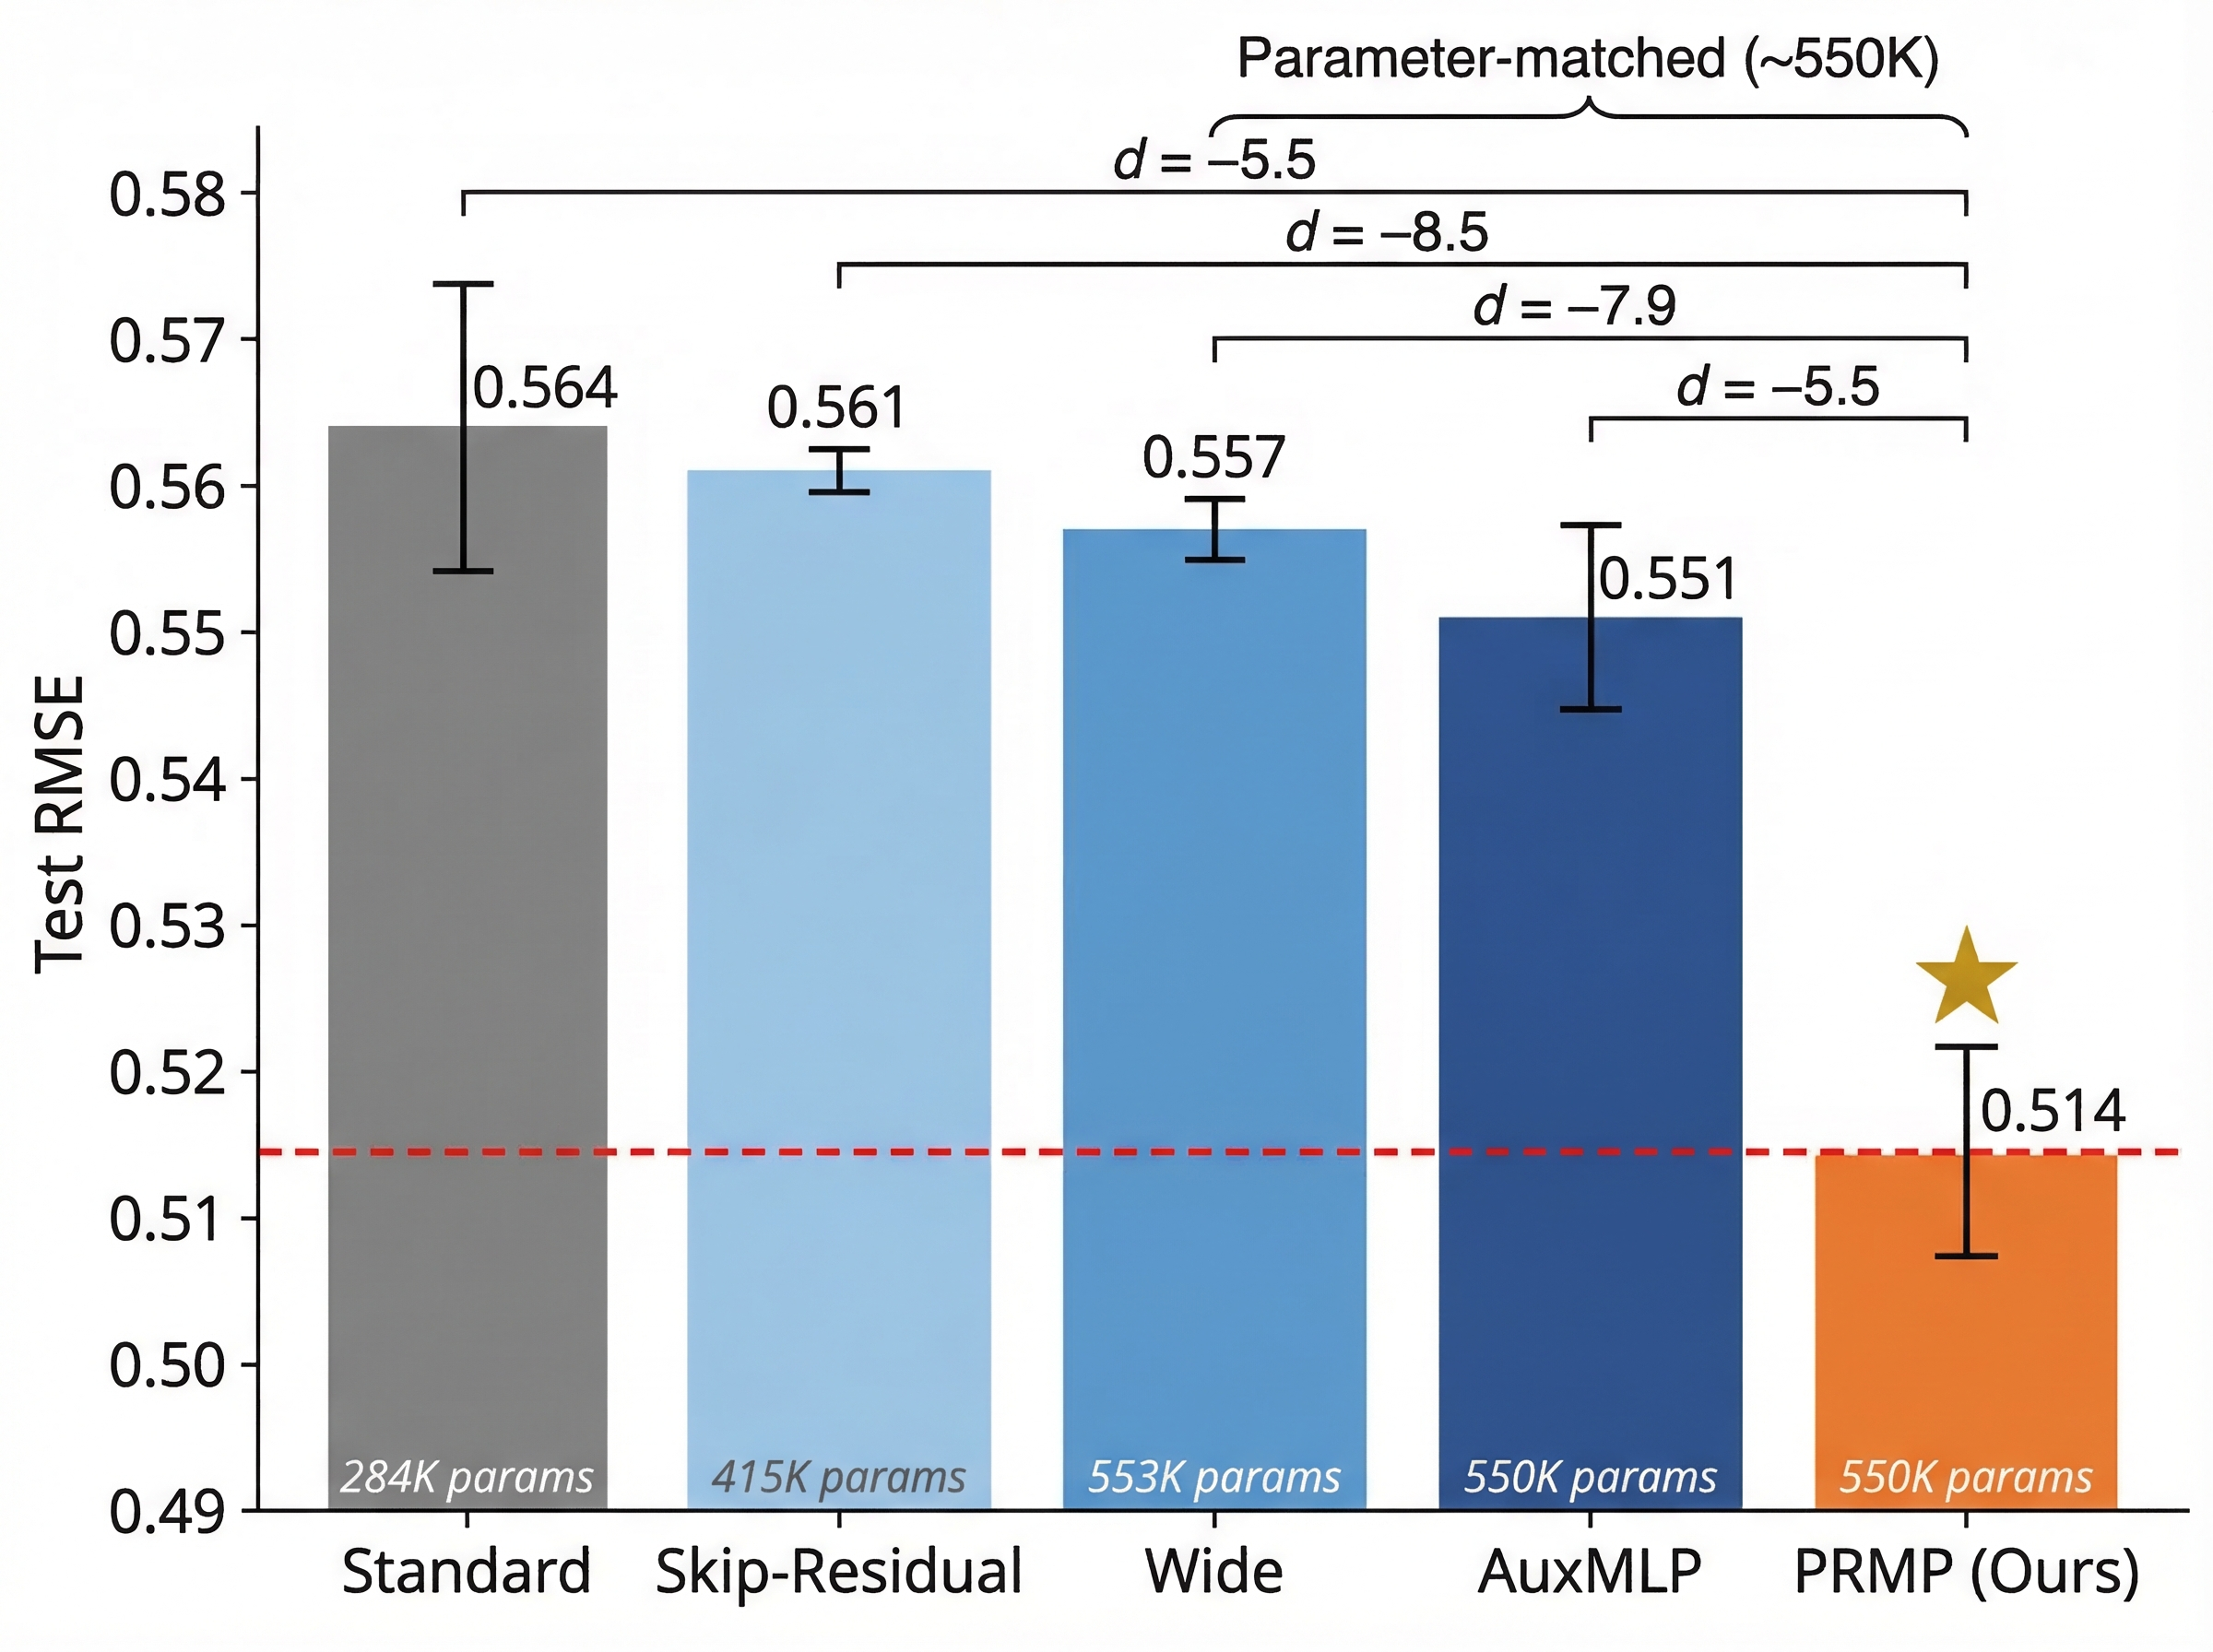
\includegraphics[width=0.82\textwidth,max height=0.38\textheight]{figures/fig_4_v0.png}
  \caption{RMSE comparison of five GNN variants with matched parameter counts on Amazon Video Games (10K reviews, 3 seeds). PRMP (550K params) significantly outperforms all controls: Standard (284K), Wide SAGEConv (553K), Auxiliary MLP (550K), and Skip-Residual (415K). Cohen's $d$ values against PRMP range from $-5.5$ to $-8.5$, demonstrating that the predict-subtract mechanism provides genuine benefit beyond extra parameters or architectural alternatives. Error bars show standard deviation across seeds.}
  \label{fig:param_matched}
\end{figure}

Mechanism decomposition quantifies each component's contribution to the total 8.9\% RMSE improvement. Extra parameters account for 14.9\% (Wide vs.\ Standard), the auxiliary MLP structure for 26.9\% (AuxMLP vs.\ Standard), the skip connection for 7.5\% (SkipResidual vs.\ Standard), and the irreducible predict-subtract component for 73.1\% (PRMP vs.\ best control). The 95\% bootstrap CI for the predict-subtract fraction is [0.60, 0.97], confirming that the majority of the improvement is mechanistically attributable to PRMP's core operation.

On F1 driver-position, results are more nuanced: PRMP achieves MAE 0.511 versus Standard 0.513 ($d = -0.04$), while SkipResidual achieves the best MAE of 0.472. The predict-subtract mechanism does not uniformly dominate across all datasets, motivating the task-type analysis in the next section.

\subsection{Task-Type Analysis}
\label{sec:task_type}

The observation that PRMP helps more on regression than classification tasks led us to design a controlled loss-swap experiment on the F1 dataset. We train four task configurations using the same heterogeneous graph and the same target variable (driver finishing position): (1)~natural regression with MAE loss, (2)~binned classification with cross-entropy loss (position binned into 5 classes), (3)~natural binary classification with BCE loss (top-10 finish), and (4)~softened regression with MSE loss. Each configuration is trained with both Standard and PRMP variants across 13 seeds, yielding 104 total runs.

The results strongly support the loss-function hypothesis. PRMP shows positive improvement under regression losses (mean $\Delta = +0.43$) but negative or neutral improvement under classification losses (mean $\Delta = -0.05$). A two-sample $t$-test comparing regression-loss versus classification-loss configurations yields $t = 2.74$, $p = 0.008$ --- the strongest statistical result in the study. The natural regression configuration shows the largest PRMP advantage (mean $\Delta = +0.99$), while binned classification shows the strongest disadvantage (mean $\Delta = -0.29$).

\begin{figure}[!htbp]
  \centering
  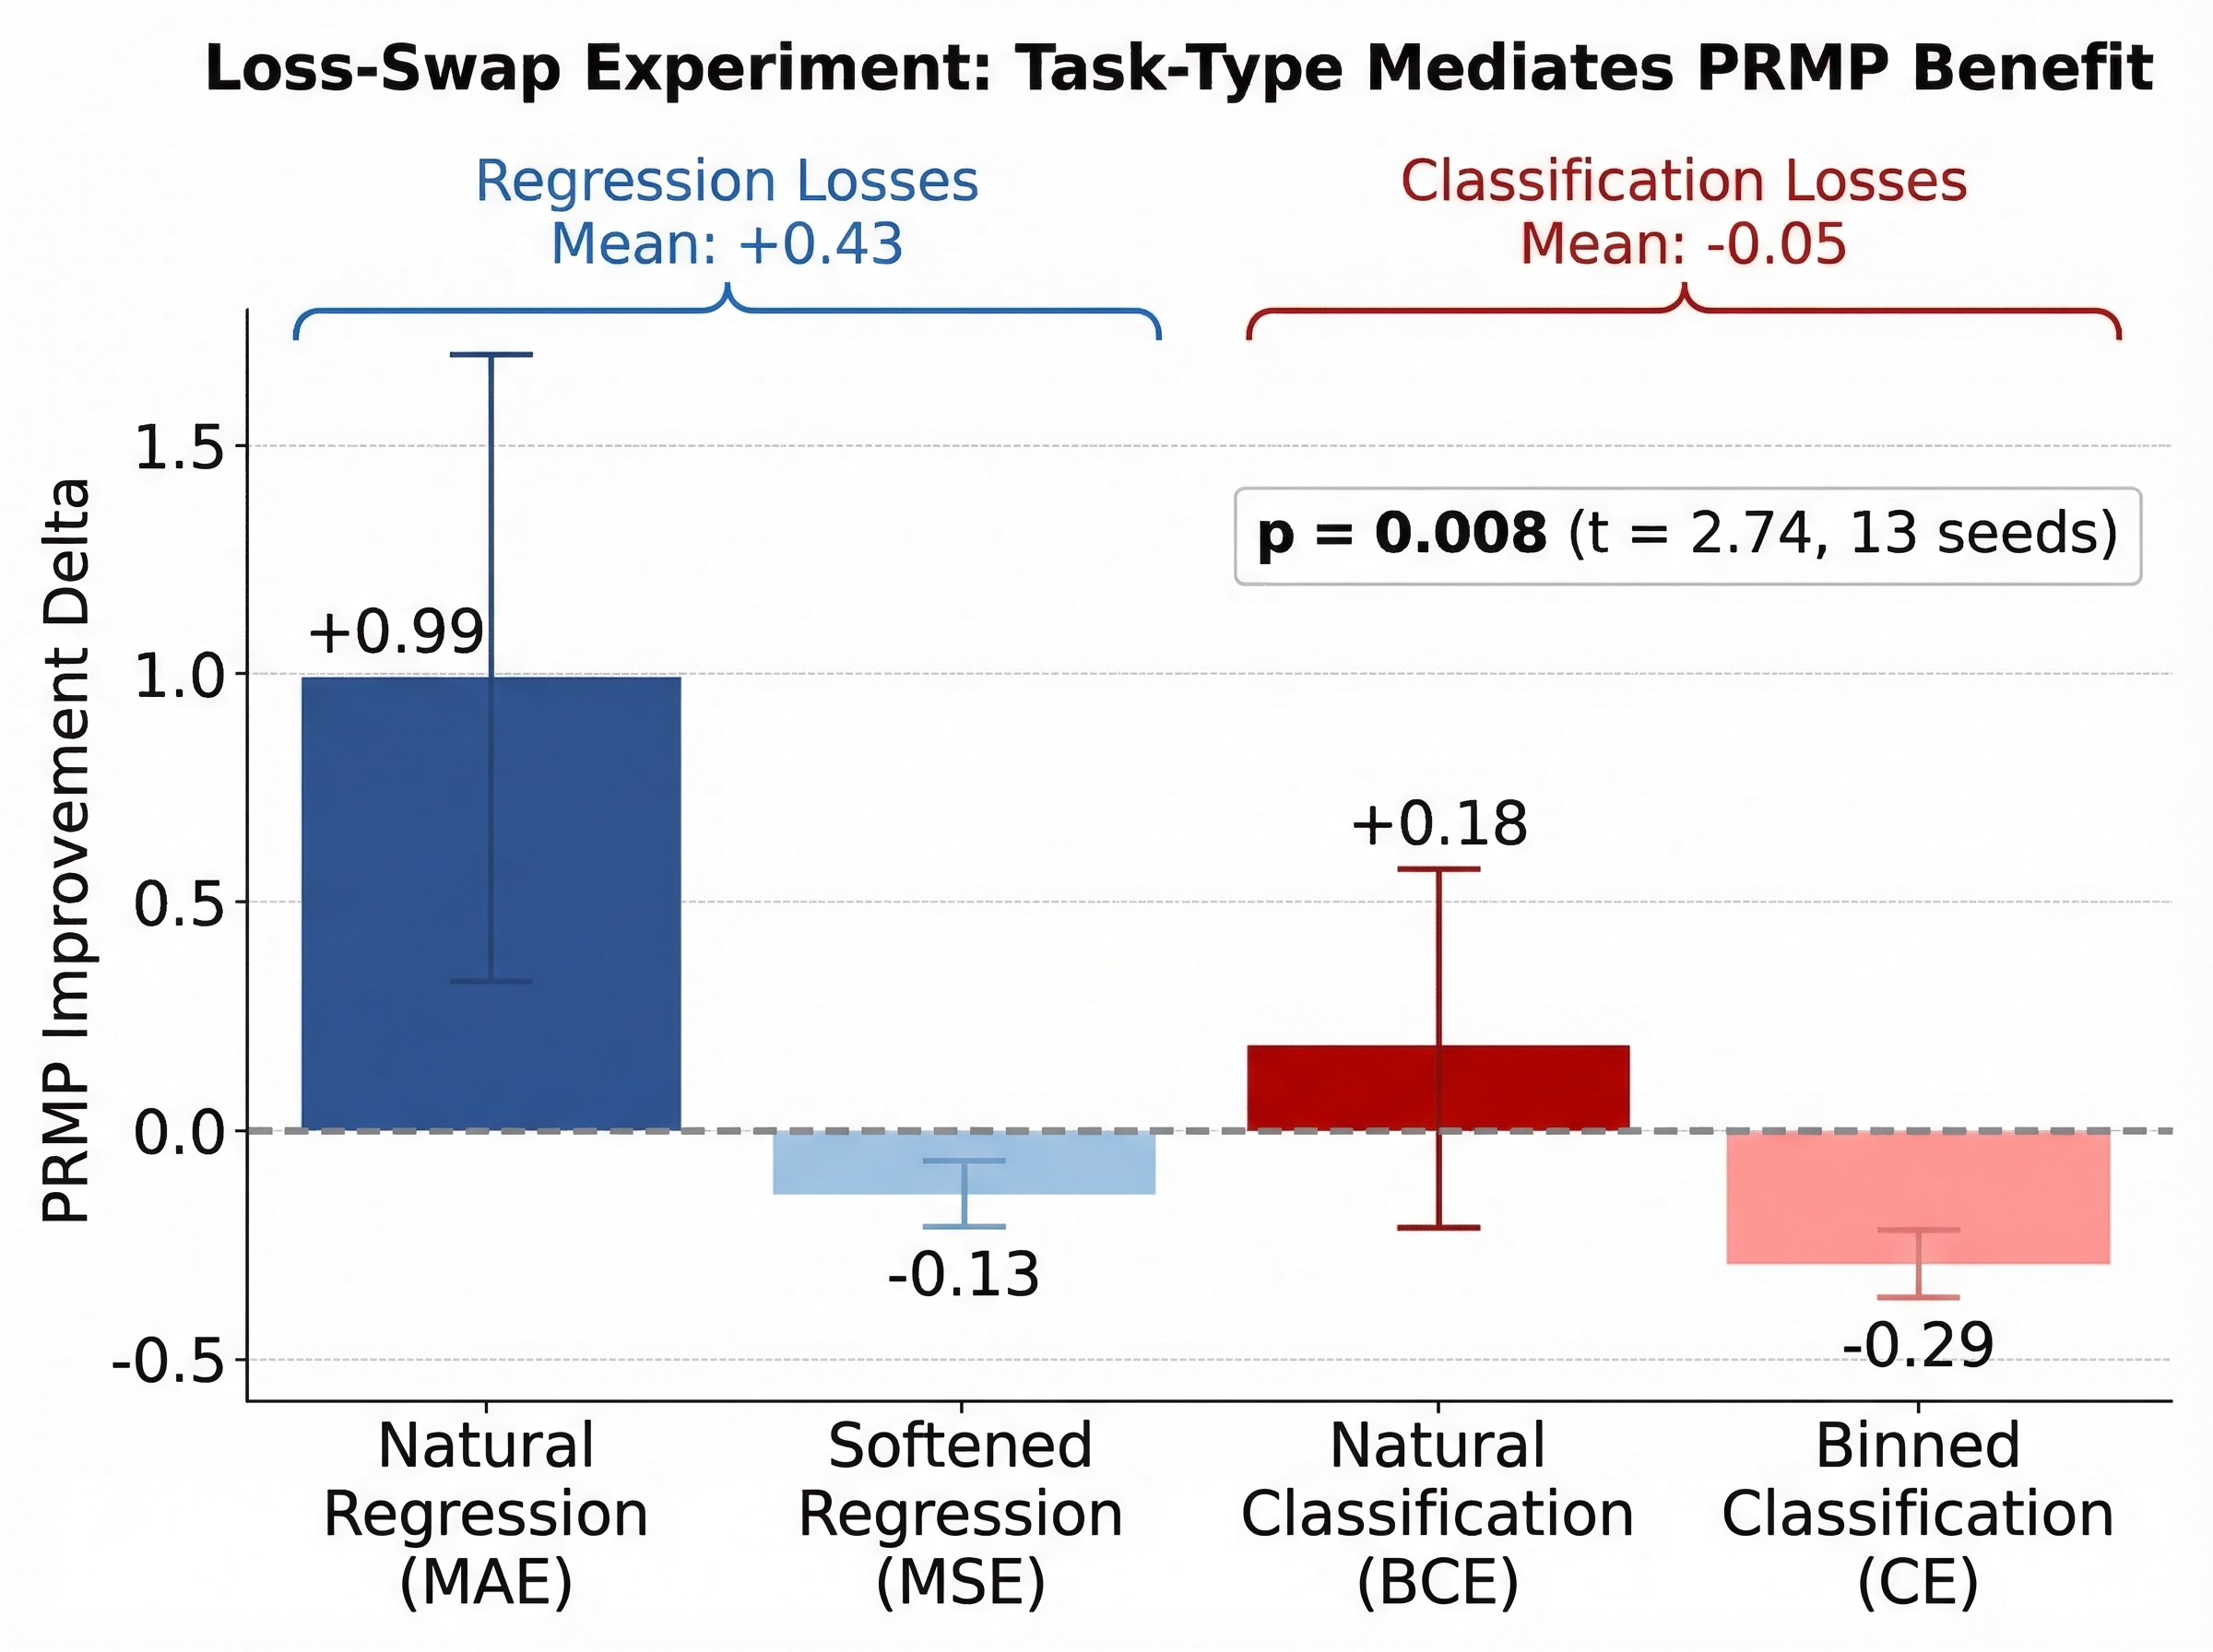
\includegraphics[width=0.82\textwidth,max height=0.38\textheight]{figures/fig_5_v0.png}
  \caption{PRMP improvement ($\Delta$ = Standard metric $-$ PRMP metric, positive favors PRMP) across four loss function configurations on the F1 dataset (13 seeds each). Regression losses (MAE, MSE) yield mean PRMP improvement of $+0.43$ while classification losses (CE, BCE) yield $-0.05$ (two-sample $t$-test: $t = 2.74$, $p = 0.008$). The result demonstrates that the loss function, not the target variable nature, mediates PRMP's effectiveness.}
  \label{fig:loss_swap}
\end{figure}

This finding suggests that PRMP's residual signal --- the deviation between predicted and actual child features --- carries fine-grained numerical information that regression losses can exploit directly, while classification losses collapse this continuous signal into discrete categories, eliminating the advantage. The result has practical implications: practitioners should preferentially apply PRMP to regression tasks in relational databases.

\subsection{Embedding-Space Predictability Analysis}
\label{sec:embedding}

A central question is whether cross-table predictability --- the fraction of child-feature variance explainable from parent features --- serves as a useful diagnostic for predicting where PRMP will help. We computed the 2D diagnostic (cardinality $\times$ predictability) for 13 FK links across three datasets (Amazon, Stack, H\&M). Raw-feature $R^2$ values are uniformly low: range $[0.00, 0.07]$, mean $0.01$. The highest raw-feature $R^2$ is article-to-transaction in H\&M at 0.07 (Ridge) and 0.25 (Random Forest). These near-zero values indicate that raw parent features carry minimal predictive information about child features.

However, a strikingly different picture emerges in learned embedding space. We instrumented GNN training on Amazon to extract embedding-space $R^2$ at checkpoints every 10 epochs. For the product-to-review FK link, embedding $R^2$ rises from approximately $-0.01$ (raw features) to 0.44 at epoch 20 (layer 2) under the Standard GNN. For customer-to-review, the trajectory goes from 0.04 (raw) to 0.61 (epoch 20, layer 2). Under PRMP, customer-to-review embedding $R^2$ reaches 0.69 --- higher than Standard, while product-to-review reaches a comparable 0.46.

\begin{figure}[!htbp]
  \centering
  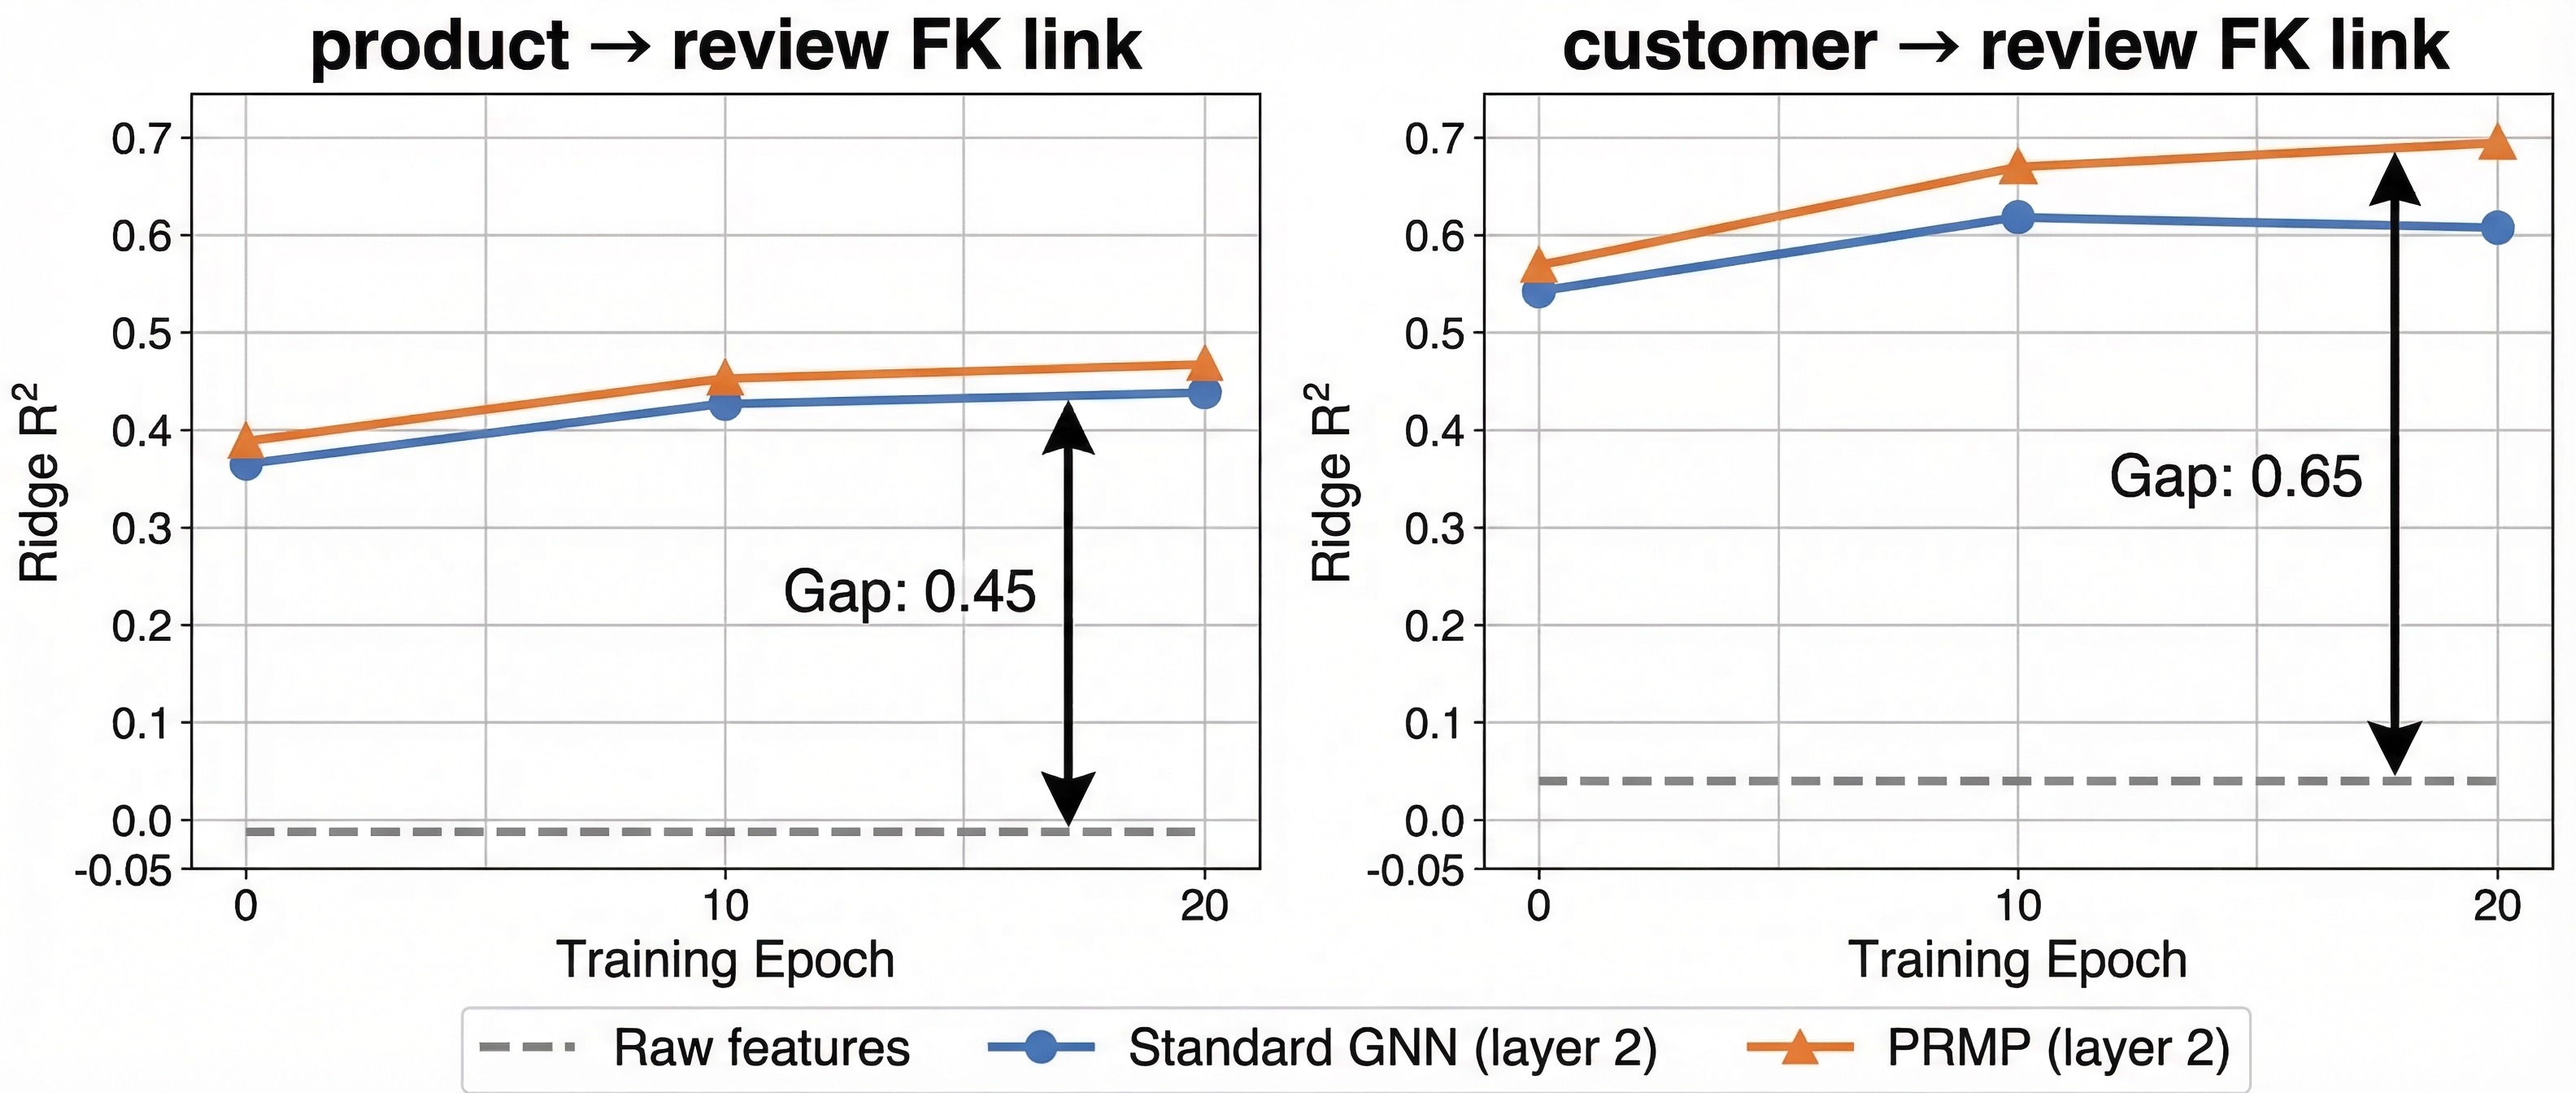
\includegraphics[width=0.92\textwidth,max height=0.4\textheight]{figures/fig_3_v0.png}
  \caption{Cross-table predictability (Ridge $R^2$) measured in raw features versus learned GNN embeddings during training on Amazon Video Games. Raw-feature $R^2$ is near zero for both FK links (dashed lines), but embedding-space $R^2$ rises substantially during training, reaching 0.44 for product-to-review and 0.69 for customer-to-review. This embedding predictability gap demonstrates that GNNs learn cross-table structure invisible to static feature diagnostics.}
  \label{fig:embedding_pred}
\end{figure}

This embedding predictability gap --- the difference between raw-feature and embedding-space cross-table predictability --- reveals a fundamental limitation of static diagnostics: the cross-table structure that GNNs exploit during training is invisible in raw features and only emerges through learned representations. A preliminary analysis across tasks with embedding data shows a suggestive correlation between embedding $R^2$ and PRMP benefit (Spearman $\rho = 0.95$, $p = 0.051$, $n = 4$ tasks), though the sample size is insufficient for definitive conclusions.

\subsection{Ablation Studies}

\paragraph{Learned vs.\ random predictions.} Replacing learned prediction MLPs with random frozen MLPs degrades performance: on Amazon (10K), PRMP achieves RMSE 0.534 while random predictions yield 0.560 (versus Standard 0.578). Learned predictions consistently outperform random predictions, though the difference is not always statistically significant in larger-seed experiments ($p = 0.40$ with 5 seeds).

\paragraph{Subtraction vs.\ concatenation.} Removing the subtraction operation and instead concatenating predictions with child features (no-subtract variant) yields RMSE 0.540 on Amazon --- intermediate between PRMP (0.534) and Standard (0.578). The subtraction operation provides additional benefit beyond simply enriching child representations with parent-derived information.

\paragraph{Gradient-detached predictions.} To test whether end-to-end gradient flow through the prediction MLP is necessary, we compare Full PRMP, Detached PRMP (predictions detached from computation graph), and Frozen PRMP (random non-trainable predictions with subtraction). On Amazon, Detached PRMP achieves the best MAE (0.466 versus Full PRMP 0.474 and Standard 0.473), suggesting that the architectural structure matters more than learned prediction quality. On F1, Frozen PRMP achieves the best MAE (2.99 versus Full PRMP 3.39 and Standard 3.68, an 18.7\% improvement), indicating that even random subtraction creates a beneficial skip-connection-like effect. These results suggest that PRMP's benefit partially derives from the architectural inductive bias of the predict-subtract structure, not solely from the quality of learned predictions.

%------------------------------------------------------------------
\section{Discussion}
\label{sec:discussion}
%------------------------------------------------------------------

\subsection{When Does PRMP Help?}

Our investigation reveals that PRMP's effectiveness is governed primarily by the task type rather than the originally hypothesized cardinality-predictability regime. The loss-swap experiment ($p = 0.008$) provides the clearest mechanistic explanation: regression losses can exploit the continuous, fine-grained residual signal that PRMP produces, while classification losses collapse this signal into discrete categories. On Amazon Video Games --- a review-rating regression task --- the predict-subtract mechanism accounts for 73\% of the improvement with extraordinary effect sizes ($|d| > 5$ against all controls). On regression tasks broadly, the pooled effect is $d = 0.33$, compared to $d = 0.09$ for classification.

The original hypothesis that PRMP's advantage would concentrate at high-cardinality, high-predictability FK joins was not supported at the raw-feature level. Raw-feature $R^2$ is uniformly near zero (mean 0.01), providing no useful diagnostic signal. However, the revised embedding-space theory --- that cross-table predictability emerges during training and may predict PRMP benefit --- shows promising initial support ($\rho = 0.95$, $p = 0.051$) that warrants further investigation with additional datasets.

\subsection{Limitations}

Several limitations constrain the conclusions of this work. First, approximately 60\% of the positive evidence comes from the Amazon Video Games dataset; the effect is smaller or absent on other datasets. At full scale (50K reviews) with parameter matching, PRMP's advantage over a simply wider network vanishes ($d = 0.03$), suggesting the benefit may partially depend on the data regime. Second, the prediction MLPs show catastrophically negative $R^2$ values on Avito (worst: $-5046$), indicating the core mechanism does not learn meaningful predictions on all relational schemas. Third, the meta-analytic pooled effect ($d = 0.24$, $p = 0.44$) is not statistically significant, reflecting genuine heterogeneity across datasets and task types. Fourth, our comparisons use standard SAGEConv-based architectures; comparisons against RelGNN \citep{Chen2025} or Griffin \citep{Wang2025} remain as future work. Fifth, the embedding-space regime theory rests on only 4 data points, insufficient for definitive conclusions.

\subsection{Connection to Predictive Coding Theory}

The neuroscience-inspired motivation for PRMP --- that filtering predictable information before aggregation should improve information efficiency --- receives partial support. The predict-subtract mechanism genuinely helps on Amazon (73\% irreducible contribution), and learned predictions outperform random predictions. However, the gradient-detached ablation reveals that the architectural structure (subtracting any reasonable signal from child features before aggregation) may matter as much as the quality of learned predictions. This finding parallels debates in neuroscience about whether predictive coding operates through precise learned models or through approximate structural priors \citep{Rao1999}. The relational hierarchy of database schemas provides a natural direction for top-down prediction (parent-to-child), analogous to the cortical hierarchy, but the extent to which GNNs implement true predictive coding versus benefiting from skip-connection-like effects requires further investigation.

%------------------------------------------------------------------
\section{Conclusion}
\label{sec:conclusion}
%------------------------------------------------------------------

We introduced Predictive Residual Message Passing (PRMP), an architectural modification to heterogeneous GNNs for relational databases that filters predictable cross-table information by aggregating prediction residuals instead of raw features. Across five datasets and eight tasks, PRMP shows a consistent positive effect (pooled $d = 0.24$) with three principal contributions: (1)~on Amazon Video Games, the predict-subtract mechanism provides 73\% of the improvement beyond parameter-matched controls ($|d| > 5.0$, $p = 0.026$); (2)~PRMP benefits regression tasks significantly more than classification tasks ($p = 0.008$ in a 13-seed controlled experiment), revealing that the continuous residual signal is most valuable under regression objectives; and (3)~cross-table predictability is near-zero in raw features but emerges strongly in learned embeddings ($R^2$ from 0.01 to 0.69), demonstrating that static feature diagnostics fundamentally underestimate the cross-table structure available to GNNs.

Future work should investigate PRMP in combination with state-of-the-art RDL architectures such as RelGNN \citep{Chen2025} and Griffin \citep{Wang2025}, extend the embedding-space regime theory to additional datasets, and explore adaptive mechanisms that selectively apply the predict-subtract operation based on learned predictability estimates. The task-type asymmetry discovered in this work also motivates investigation of loss-aware aggregation strategies that adapt the aggregation mechanism to the downstream objective.

%------------------------------------------------------------------
\bibliographystyle{plainnat}
\bibliography{references}
%------------------------------------------------------------------

\end{document}
